\documentclass{acm_proc_article-sp}
\usepackage[utf8]{inputenc}

\renewcommand{\paragraph}[1]{\vskip 6pt\noindent\textbf{#1 }}
\usepackage{hyperref}
\usepackage{graphicx}
\usepackage{url}

\providecommand{\tightlist}{%
  \setlength{\itemsep}{0pt}\setlength{\parskip}{0pt}}

\title{Visualization for Visualization (VIZfVIZ)}


% Add imagehandling

\numberofauthors{2}
\author{
\alignauthor Xinyue Bai \\
        \affaddr{}\\
       \email{}
\and \alignauthor Weimin Zhang \\
        \affaddr{}\\
       \email{}
\and \alignauthor Hongting Li \\
        \affaddr{}\\
       \email{}
\and }

\date{}

%Remove copyright shit
\permission{}
\conferenceinfo{} {}
\CopyrightYear{}
\crdata{}

% Pandoc syntax highlighting

% Pandoc citation processing
\newlength{\csllabelwidth}
\setlength{\csllabelwidth}{3em}
\newlength{\cslhangindent}
\setlength{\cslhangindent}{1.5em}
% for Pandoc 2.8 to 2.10.1
\newenvironment{cslreferences}%
  {}%
  {\par}
% For Pandoc 2.11+
\newenvironment{CSLReferences}[3] % #1 hanging-ident, #2 entry spacing
 {% don't indent paragraphs
  \setlength{\parindent}{0pt}
  % turn on hanging indent if param 1 is 1
  \ifodd #1 \everypar{\setlength{\hangindent}{\cslhangindent}}\ignorespaces\fi
  % set entry spacing
  \ifnum #2 > 0
  \setlength{\parskip}{#2\baselineskip}
  \fi
 }%
 {}
\usepackage{calc} % for calculating minipage widths
\newcommand{\CSLBlock}[1]{#1\hfill\break}
\newcommand{\CSLLeftMargin}[1]{\parbox[t]{\csllabelwidth}{#1}}
\newcommand{\CSLRightInline}[1]{\parbox[t]{\linewidth - \csllabelwidth}{#1}}
\newcommand{\CSLIndent}[1]{\hspace{\cslhangindent}#1}


\begin{document}
\maketitle

\begin{abstract}
Where does the data visualisation stands today? Collected and organized
by Data Visualization Society, Annual Data visualization Community
Survey includes 50+ data visualization related questions and covers data
visualization details such as salary, tool usage, demographic data,
audiences and organizational structure. This survey provides valuable
insights for organizations, practitioners and people who love data
visualisation. As three university students passionate about data
visualisation, the objective of this project is to design and develop an
interactive R Shiny application to allow audiences to explore data
visualisation community survey data, and to maximise the insights
obtained from the survey data. We demonstrate survey result from 3
dimensions, interactive exploratory data analysis, cluster analysis and
association analysis. Application's design framework and project
findings are also discussed.
\end{abstract}

\hypertarget{introduction-and-motivation-of-the-application}{%
\section{1 Introduction and Motivation of the
application}\label{introduction-and-motivation-of-the-application}}

Data visualization is the graphical representation of information and
data. It has been an important factor in data analytics pipeline, to
reveal insights that are often difficult to be delivered in other forms.
It is commonly used in various scenarios, such as data cleaning,
exploring data structure, detecting pattern, identifying trends and
clusters. It provides organizations and practitioners a handy tool to
analyse data and enables them to make informative decisions based on
insights gained. Understanding the current state of data visualization
is crucial. It gives organizations and practitioners in the field a
better idea of where data visualization stands today, and where it's
headed. On the other hand, it helps people who have an interest in data
visualization know how to enter the field.

\hypertarget{objective}{%
\section{2 Objective}\label{objective}}

In this research study, we will build a R Shiny application to
illustrate the current trend of data visualization. The goal is to draw
a comprehensive picture of data visualization for organizations,
practitioners and people having an interest in data visualization, by
analysing Annual Data visualization Community Survey. The analysis and
visualization consist of three parts: interactive exploratory data
analysis, cluster analysis and association analysis. • The exploratory
data analysis aims to summarize the main characteristics of the measures
and generate statistical graphics to visualize them. • The cluster
analysis aims to discover similarities in respondents based on tools
they used and hours they spent on data visualisation; to group data
visualisation tools and visualisation activities. • The association
analysis aims to provide DataViz practitioners a guidance what are the
commonly used combination of tools.

\hypertarget{review-and-critic-on-past-works}{%
\section{3 Review and Critic on Past
Works}\label{review-and-critic-on-past-works}}

Duis nec purus sed neque porttitor tincidunt vitae quis augue. Donec
porttitor aliquam ante, nec convallis nisl ornare eu. Morbi ut purus et
justo commodo dignissim et nec nisl. Donec imperdiet tellus dolor, vel
dignissim risus venenatis eu. Aliquam tempor imperdiet massa, nec
fermentum tellus sollicitudin vulputate. Integer posuere porttitor
pharetra. Praesent vehicula elementum diam a suscipit. Morbi viverra
velit eget placerat pellentesque. Nunc congue augue non nisi ultrices
tempor.

\hypertarget{interactive-exploratory-data-analysis-ieda}{%
\subsection{3.1 Interactive Exploratory Data Analysis
(IEDA)}\label{interactive-exploratory-data-analysis-ieda}}

In statistics, exploratory data analysis is an approach to analyze data
sets to summarize their main characteristics. We are going to use
statistical graphics to visualize the results of IEDA. Past works
focused on numerical variables and explored different facility provided
by the ``ggplot'' package.\\
There are two main areas to improve.Hadley (n.d.) 1. The focus on
``ggplot'' package does not provide interactivity. 2. The focus on
numerical variables restricted the scenarios that the results could be
applied to.

\hypertarget{latent-class-analysis}{%
\subsection{3.2 Latent Class Analysis}\label{latent-class-analysis}}

Since this is a survey data, columns in the dataset all have categorical
variables. It's not appropriate to use clustering techniques such as
dendrogram and k-means clustering method. Instead, Latent class analysis
(LCA), which was commonly used for the analysis of multivariate
categorical data, is taken into considerations in this case. LCA offers
a way to uncover hidden groupings (latent classes) in multivariate
categorical data, by applying maximum likelihood method to calculate the
probability that a case will fall in a particular latent class. This
unsupervised clustering algorithm can be achieved by poLCA package in R.
In a research paper written by Linzer and Lewis, they had illustrated
multiple examples of LCA with detailed explanation in R, using built-in
carcinoma, cheating, election, gss82 and values dataset
(\textbf{LL2011?}). However, they did not visualise the output of LCA.
In this project, ggplot2, plotly and heatmaply packages were used to
visualise LCA's outputs, class-conditional outcome probabilities
(LCAoutput\(probs) and each observation’s posterior class membership probabilities (LCAoutput\)posterior).

\hypertarget{association-analysis}{%
\subsection{3.3 Association Analysis}\label{association-analysis}}

\hypertarget{association-rule-mining}{%
\subsubsection{3.3.1 Association rule
mining}\label{association-rule-mining}}

Association rule mining is rule-based method to discover association
between different objects in a set, and frequent patterns in a database.
Commonly used terminologies in association analytics include itemset,
support, confidence, lift, whereas, - Itemset is one item or combination
of items. K-itemset means an itemset with k items. One instance of
itemsets is typically called a ``transaction.'' - Frequency percentage
of X over total number of transaction records, N. Support (X) =
frequency(X)/N\\
- For a rule A=\textgreater B, confidence shows percentage in which B
occurs when A occurs. -
Confidence(A=\textgreater B)=P(A∩B)/P(A)=frequency(A,B)/frequency(A) -
Lift gives correlation between A and B in the rule A=\textgreater B.
Correlation shows how one item-set A effects the item-set B. Lift of 1
represents independence between A and B. Larger than 1 means presence of
A gives positive effect and less than 1 represent negative effect.

APRIORI algorithm is used for association rule mining. It starts with
frequent itemset generation and find all frequent item-sets satisfy
pre-determined min-support threshold. List all association rules from
frequent item-sets. Calculate support and confidence for all rules and
keep rules that satisfy min\_support and min\_confidence threshold. For
each rule, we can use lift to examine the correlation of itemset A and
itemset B.(Agrawal and Srikant 1994)

Association rule mining is popularly implemented with R extended
packages, arules.(Hahsler et al. 2021) It always generate a large number
of association rules. Researchers have developed, studied, and
implemented novel methods to visualize the result with ``arulesViz.'' It
does not only support common association visualization types
e.g.~``scatterplot,'' ``matrix'' and ``graph,'' also support ``two-key
plot,'' ``matrix3D,'' ``mosaic,'' ``doubledecker,'' ``paracoord,''
``grouped,'' and also an interactive component ``ruleExplorer.''
(Hahsler 2021) Researchers have studied association rule visualization
with hierarchical groups.(Hahsler 2017) However, it comes to a
limitation to explore the association for a subgroup of the
transactions, by filtering multiple parallel information.

This study target to customize existing ruleExplorer function with
additional interactivity component to focus on selected subgroup. Our
first iteration flow is to read file into R, followed by filtering and
saving selected data, and then read into R as transactions. However,
every filtering would trigger a temporary file at the server side, which
is very time and capacity consuming. The proposed iteration is by
incorporating itemset level information using functions from arules.

\hypertarget{parallel-sets-a-novel-approach-to-compare-multiple-item-sets-information}{%
\subsubsection{3.3.2 Parallel Sets -- a novel approach to compare
multiple item sets
information}\label{parallel-sets-a-novel-approach-to-compare-multiple-item-sets-information}}

Parallel sets marry the advantages of two visualisation techniques,
parallel coordinates which can display high-dimensional data and using
frequencies to represent for the categories. In parallel sets, the width
of box between two dimensions reflects the percentage of different
category. In R, interactive parallel sets can be achieved by parsetR
package. This is a software package built upon R Shiny and its
functionalities are quite straightforward.

In the previous work of Kosara, Bendix and Hauser, a customer survey
dataset, containing information about 93,872 Austrian households, was
used in their case study (Linzer and Lewis 2011). They deployed parallel
sets to illustrate three dimensions that are of particular interest:
household types, income and favourite supermarket. The result chart is
shown below. Particularly, a histogram was plotted in the middle,
showing the frequency distribution of the top and bottom dimensions
relative to the middle dimension. In comparison to the demonstration in
this case study, parsetR package does not include statistical
information on the plot. It would be good if this functionality can be
incorporated in parsetR package.

\begin{center}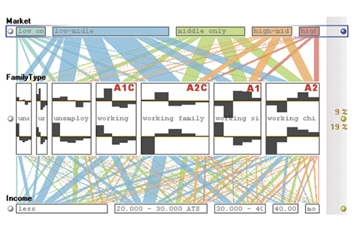
\includegraphics[width=1\linewidth]{1} \end{center}

\hypertarget{design-framework-and-use-case-demonstration}{%
\section{4 Design framework and Use Case
Demonstration}\label{design-framework-and-use-case-demonstration}}

On the top of the interface, we provide a navigation header that enables
users to select the analysis they would like to explore -- Interactive
exploratory design analysis, clustering or association analysis.

\hypertarget{interactive-exploratory-data-analysis-ieda-1}{%
\subsection{4.1 Interactive Exploratory Data Analysis
(IEDA)}\label{interactive-exploratory-data-analysis-ieda-1}}

A drop-down menu is provided under the IDEA header button, which enable
the users to select one of the subjects in Demography information, Job
and Challenge faced. Once selected, the application will jump to an
interface built for that subject. On this interface, a control panel on
the left side provides the interactivity for users to select the
variable they would like to examine and the variable they would like to
group the data. Once selected, a bar chart with error bar will be
generated to present the proportion of each value of the variable
examined.

\begin{center}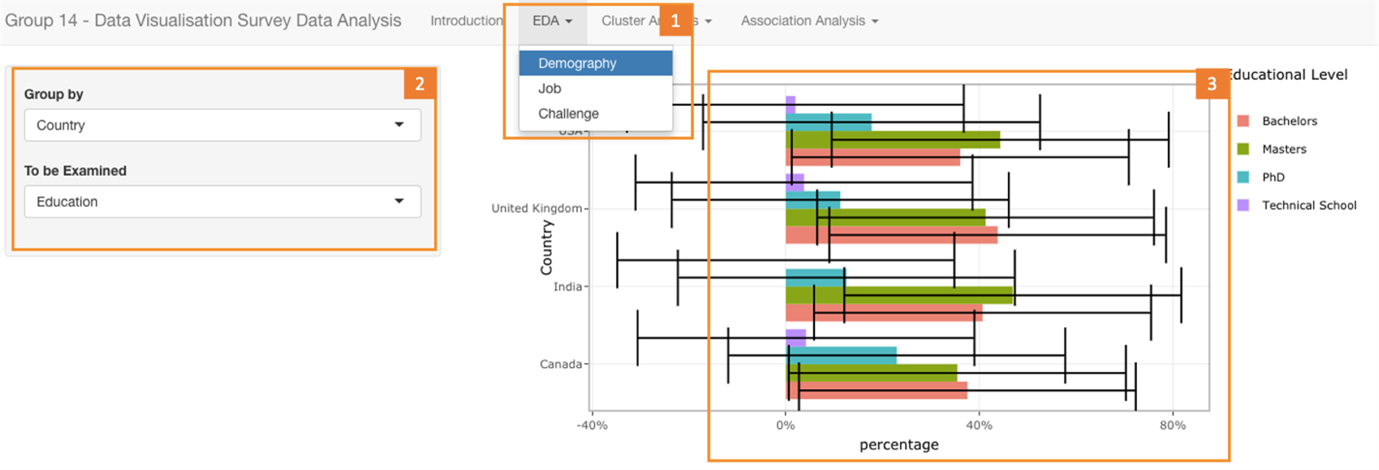
\includegraphics[width=1\linewidth]{2} \end{center}

\hypertarget{cluster-analysis}{%
\subsection{4.2 Cluster Analysis}\label{cluster-analysis}}

Cluster analysis contains four parts as shown below: 1. On the menu bar,
Latent Class Analysis is available under Cluster Analysis section. 2.
For Latent Class Analysis section, three visualisation variations, line
plot, stacked bar chart and heatmap, are available for selection. Same
data is used for all three different formats. Line plot and stacked bar
chart aims to cluster variables, in order to find out what tools belong
to the same group and the relationship between varied duration of
working on different visualisation tasks, whereas heatmap cluster
respondents based on their behaviours (i.e.~tools used and hours spent).
3. For each visualisation format of LCA, slider bar on the left contains
a slider input for number of classes. As only 10 frequently-mentioned
visualisation tools are included for cluster analysis after data
pre-processing, the range of classes available for selection is between
1 and 9. Users can adjust number of clusters to observe the changes and
find optimal number of classes, by moving the circle button. 4. Apart
from number of classes available for selection, there are two groups of
cluster variables. The first group looks into visualisation tools, which
includes Excel, Tableau, R, ggplot2, D3, Python, Pen\&Paper,
Illustrator, PowerBI and Plotly. With these variables, tools will be
clustered into different groups based on respondents' usage of tools.
The second group focuses on hours spent on different data-related
activities. More specifically, it considers hours spent on data
visualisation, data engineering, data science, design, data preparation
and building portfolio.

\begin{center}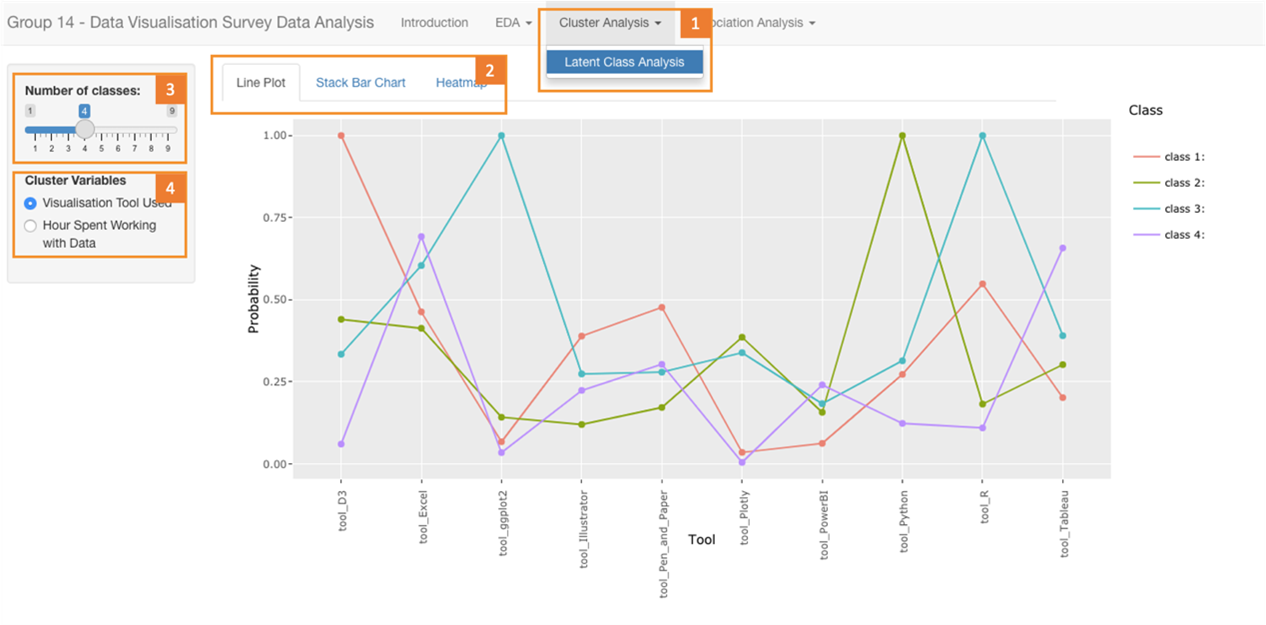
\includegraphics[width=1\linewidth]{3} \end{center}

\hypertarget{association-analysis-1}{%
\subsection{4.3 Association Analysis}\label{association-analysis-1}}

\hypertarget{association-analysis-2}{%
\subsubsection{4.3.1 Association
Analysis}\label{association-analysis-2}}

Association Rule Explorer contains four parts as displayed below: 1. On
the left side, it contains multiple demographics selector, using ,
e.g.~education, year of relevant DataViz experience, major, gender,
country and salary. After selecting from various dropdown lists and
sliderbar, user is required to click ``GO!'' button to generate subset
of transactions and thereafter charts. 2. At the middle, there is a
ruleExplorer built-in interactive component, which allows user to filter
measures (i.e.~minimum support, confidence, lift), rule length, and
inclusive and/or exclusive items. 3. At the right top corner, it is also
a ruleExplorer built-in interactive tabbar. This offers various
visualization output types. 4. Last but not least, area \#4 will ideally
display selected output chart with desired subset of transactions and
satisfying rules.

\begin{center}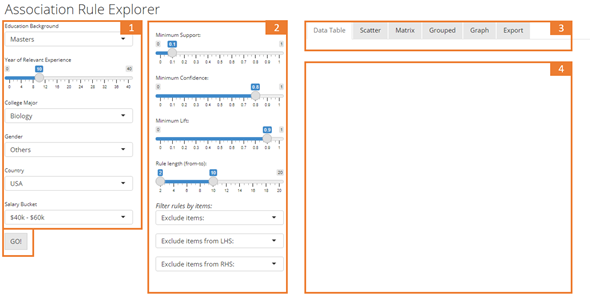
\includegraphics[width=1\linewidth]{4} \end{center}

\textbf{(disclaimer: above proposed design is not implemented
successfully.)}

\hypertarget{parallel-set-chart}{%
\subsubsection{4.3.2 Parallel Set Chart}\label{parallel-set-chart}}

Parallel set contains two parts as illustrated below: 1. On the menu
bar, Parallel Set Chart is available under Cluster Analysis section. 2.
Slider bar on the left contains two selection inputs. This allows users
to select variables of interest and explore the relationship between two
variables, such as role of respondents in organization and usage of tool
Excel, or usage of tool Tableau and tool R. Variables consist of
undergraduate major, organization area, role, gender, country, yearly
pay, Excel, Tableau, R, ggplot2, D3, Python, Pen\&Paper, Illustrator,
PowerBI and Plotly.

\begin{center}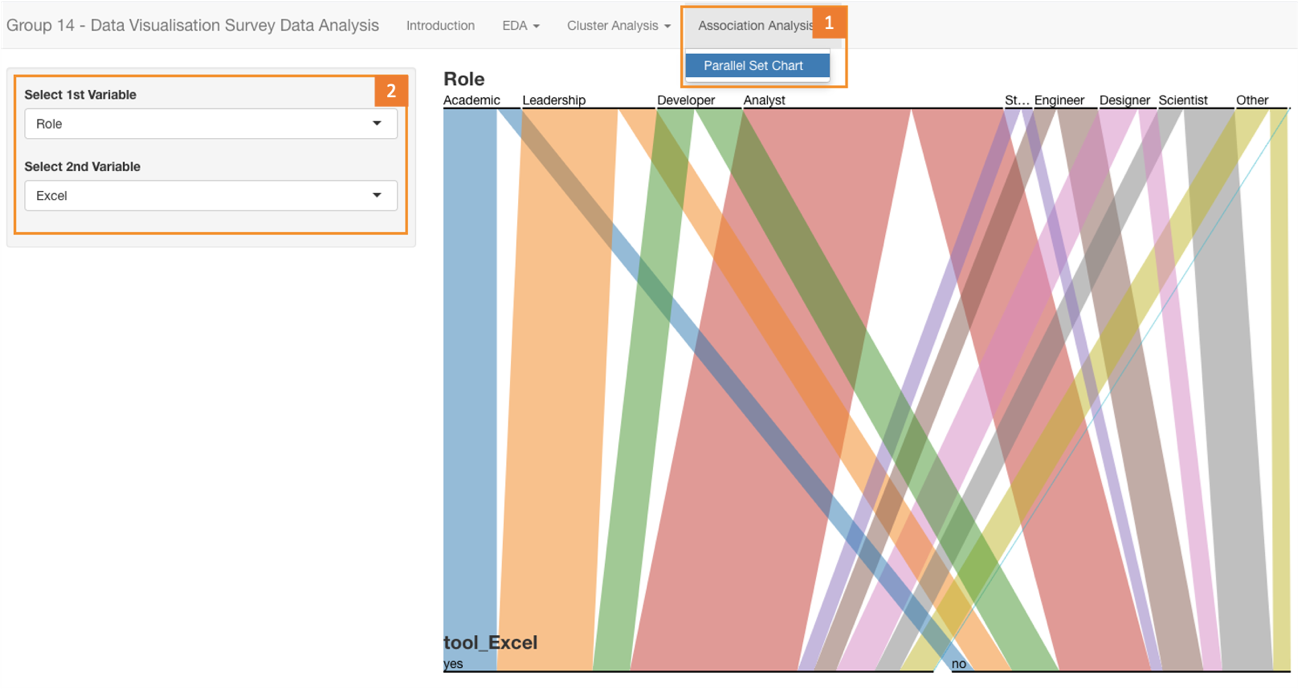
\includegraphics[width=1\linewidth]{5} \end{center}

\hypertarget{discussion}{%
\section{5 Discussion}\label{discussion}}

In this project, we have explored functions of different R packages to
visualize categorical variables. Our R Shiny application incorporates
interactivity and provides an application case that is useful for
exploring and presenting categorical data.

\hypertarget{bar-chart-1}{%
\subsection{5.1 Bar Chart 1}\label{bar-chart-1}}

Generally, there more male data visualisation professionals. India has
the largest gap between the number of male data visualisation
professionals and the that of female professionals (81\%male vs.19\%
female). USA has the smallest gap between the number of male data
visualisation professionals and the that of female professionals 62\%
male vs.39\% female).

\begin{center}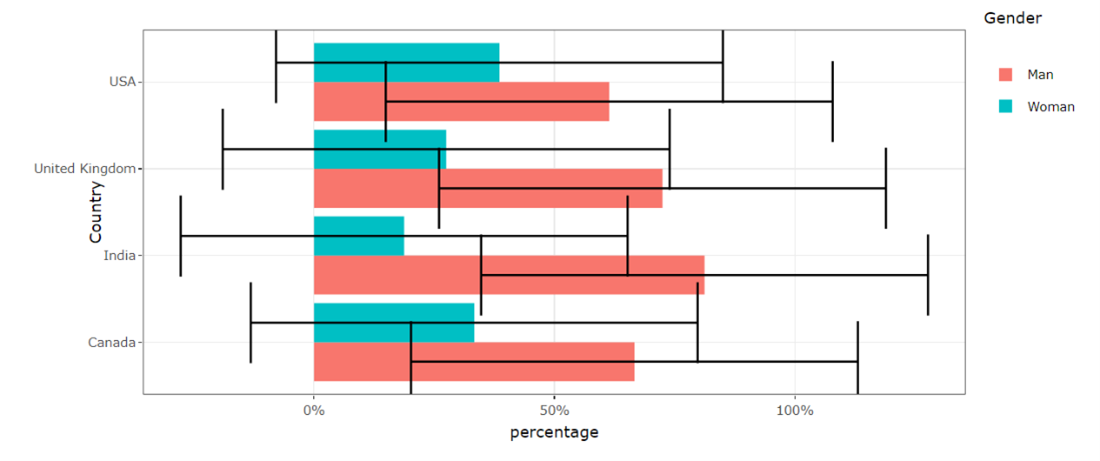
\includegraphics[width=1\linewidth]{7} \end{center}

\hypertarget{bar-chart-2}{%
\subsection{5.2 Bar Chart 2}\label{bar-chart-2}}

Private sector requires and employed highest portion, more than 40\%, of
dataViz practitioners across USA, UK, India and Canada. This is followed
by academic instituitions.

\begin{center}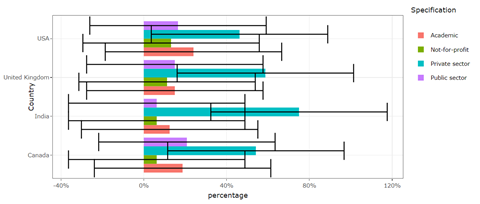
\includegraphics[width=1\linewidth]{9} \end{center}

\hypertarget{lca---heatmap}{%
\subsection{5.3 LCA - Heatmap}\label{lca---heatmap}}

Heatmap allows users to visually capture different groups in survey
respondents, based on their usage of visualisation tools. Originally,
it's difficult to use heatmap to visualise categorical data. With
posterior probabilities computed from LCA, we are able to cluster
respondents into different latent classes and clearly show the groupings
on heatmap. Besides, hovering over the plot can see ID of respondents.
Thus, an interactive heatmap helps us locate respondent easily.

\begin{center}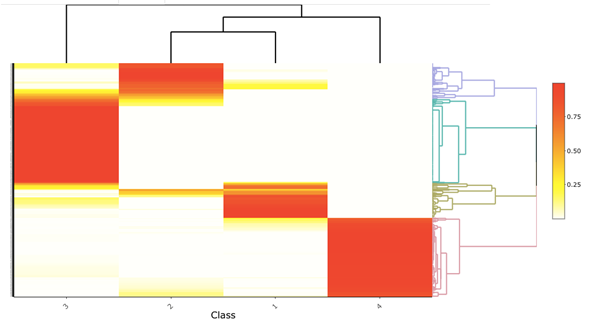
\includegraphics[width=1\linewidth]{11} \end{center}

\hypertarget{lca-line-plot}{%
\subsection{5.4 LCA -- Line Plot}\label{lca-line-plot}}

Line plot provides users with a more complete picture of the cluster
result, as probabilities of belonging to all different classes are all
presented on the graph. Besides, it's easy to detect whether two
categories are from the same group, by observing the trend of the graph.
In the example shown below, we can see that ggplot2 and R are highly
likely from the same class, class 2. This is obvious looking at the peak
of green line and this grouping is reasonable since ggplot2 is a
commonly used R package.

\begin{center}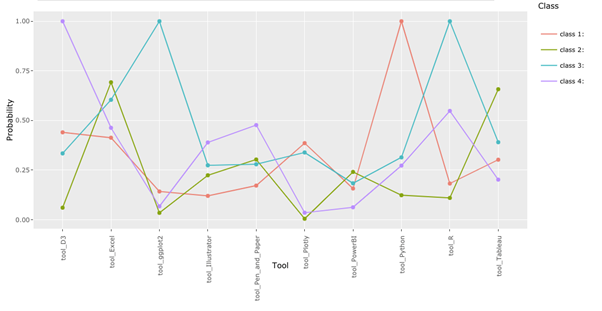
\includegraphics[width=1\linewidth]{12} \end{center}

\hypertarget{lca-stacked-bar-chart}{%
\subsection{5.5 LCA -- Stacked Bar Chart}\label{lca-stacked-bar-chart}}

100\% Stacked bar chart shows the percentage of every sub-category in
relation to the total value. This allows users to spot the largest
sub-category easily and the difference between sub-categories. According
to the below example, python and R belong to very different classes.
This is because when using R has 100\% probability in class 1, the
probability of using python is small, whereas when using python is 100\%
probability in class 3, the probability of using R is very low.

\begin{center}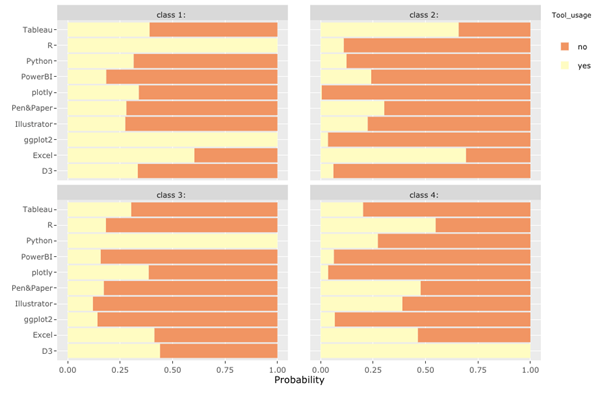
\includegraphics[width=1\linewidth]{13} \end{center}

\hypertarget{association-analysis-3}{%
\subsection{5.6 Association Analysis}\label{association-analysis-3}}

Association rules can help dataViz tool providers to advertise and cross
sell products to users who used associated product. It can also help
dataViz practitioners to learn new set of tools that be skilled by
others. From below chart with a low lift, we can see that the
association is quite sparse, there is no clear group of tools that be
used by a cluster of users, i.e dataViz practitioners have diverse
experience with different set of tools.

\begin{center}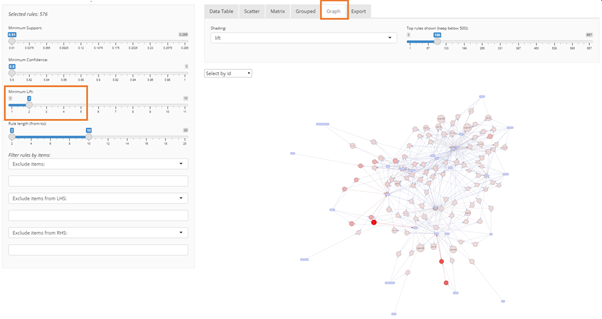
\includegraphics[width=1\linewidth]{14} \end{center}

The proposed design allows user to select measures such as minimum lift,
which shows rules with larger lift, i.e.~more significant positive
effect for association.

\begin{center}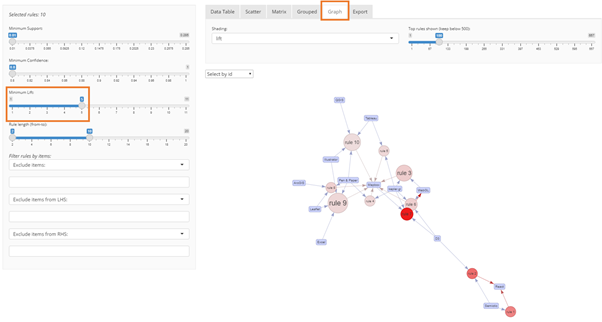
\includegraphics[width=1\linewidth]{15} \end{center}

\hypertarget{future-work}{%
\section{6 Future Work}\label{future-work}}

We have successfully implemented proposed design in terms of EDA and
Cluster Analysis. However, association analysis component is not. We
started the first iteration with a Load (raw data)-Transform (clean and
filter)-Export\&2nd Transform (to transactions)-2nd Load(as
transactions) cycle, which triggers a file saving when there is filter
change on demographics input. It is very time and capacity-consuming,
and the saved file failed to locate to a defined location and caused
issue at 2nd loading phase. Then, we did second iteration to offline
Load(raw data)-Transform (clean)-Export (to transactions and itemset
level labels), followed by a Load(transactions and itemset level
information) on ShinyAPP. We should continue to explore and extend our
study on 2nd iteration to visualize association rules.

\hypertarget{references}{%
\subsection{\# 7 References}\label{references}}

\ldots{}

\hypertarget{refs}{}
\begin{CSLReferences}{1}{0}
\leavevmode\hypertarget{ref-agrawal1994}{}%
Agrawal, Rakesh, and Ramakrishnan Srikant. 1994. {``Fast Algorithms for
Mining Association Rules in Large Databases.''} \emph{Proceedings of the
20th International Conference on Very Large DATA Bases, IBM Research
Report} 94.

\leavevmode\hypertarget{ref-HADLEY}{}%
Hadley. n.d. \emph{Exploratory Data Analysis}.
\url{https://r4ds.had.co.nz/exploratory-data-analysis.html}.

\leavevmode\hypertarget{ref-michael2017}{}%
Hahsler, Michael. 2017. {``Visualizing Association Rules in Hierarchical
Groups.''} \emph{Journal of Business Economics} 87.
\url{https://doi.org/10.1007/s11573-016-0822-8}.

\leavevmode\hypertarget{ref-R-arulesViz}{}%
---------. 2021. \emph{arulesViz: Visualizing Association Rules and
Frequent Itemsets}. \url{https://github.com/mhahsler/arulesViz}.

\leavevmode\hypertarget{ref-R-arules}{}%
Hahsler, Michael, Christian Buchta, Bettina Gruen, and Kurt Hornik.
2021. \emph{Arules: Mining Association Rules and Frequent Itemsets}.
\url{https://github.com/mhahsler/arules}.

\leavevmode\hypertarget{ref-KBH2006}{}%
Linzer, Drew A, and Jeffrey B Lewis. 2011. {``poLCA: An r Package for
Polytomous Variable Latent Class Analysis.''} \emph{Journal of
Statistical Software} 42.

\leavevmode\hypertarget{ref-William2017}{}%
Surles, William. 2017. \emph{Exploratory Data Analysis in r: Case
Study}. \url{https://rpubs.com/williamsurles/299664}.

\end{CSLReferences}
\setlength{\parindent}{0in}

\end{document}
